% \section{Named Entity Extraction} 

% Extracting named entities from texts and representing them as nodes in knowledge graphs generally, involves three main
% tasks: Named Entity Recognition (NER), Named Entity Disambiguation (NED) and Named Entity Linking (NEL). 

\section{Named Entity Recognition (NER)} \label{named_ents}

Named entity recognition (NER) is a process which extracts and classifies named entities of certain (pre-defined) types such as `PER' (person), `GPE' (geo-political entities), `ORG' (organisation) from an unstructured text~\cite{ieee_named_entity}Refer to Appendix~\Cref{appendix:semantic_types} for the full list of entity types used by AllenNLP and spaCy. 

First, it identifies the `names' of the entities from the pre-processed tokens commonly done by BILOU tagging (See~\Cref{bilou}) and POS tagging. It then performs sequence labelling (assigning labels/tags to each element of an input sequence) and classifies entities into the predefined types such person, location, organisation and so on~\cite{ieee_named_entity}. \Cref{fig:bilou} highlights how the Named Entity Recognition process uses BILOU scheme to extract a ORG `Imperial College London' and GPE: `London'.

\begin{table}[H]
    \centering 
    \renewcommand{\arraystretch}{1.1}
    \begin{tabularx}{0.7\textwidth}{|>{\hsize=.1\hsize\linewidth=\hsize}X|>{\hsize=.2\hsize\linewidth=\hsize}X|>{\hsize=.6\hsize\linewidth=\hsize}X|} 
    \hline
    \textbf{Tag} & \textbf{Meaning} &\textbf{Description}  \\
    \hline
    \textbf{B} & Beginning & First token of a multi-token entity\\
    \textbf{I}  & Inside & An inner token of a multi-token entity\\
     \textbf{L}  & Last & Final token of a multi-token entity\\
     \textbf{O}  & Outside & A single-token entity\\
     \textbf{U} & Unit & A non-entity token\\
     \hline
    \end{tabularx}
\caption{BILOU tagging scheme}
\label{bilou}
\end{table}

\begin{figure}[H]
    \centering
    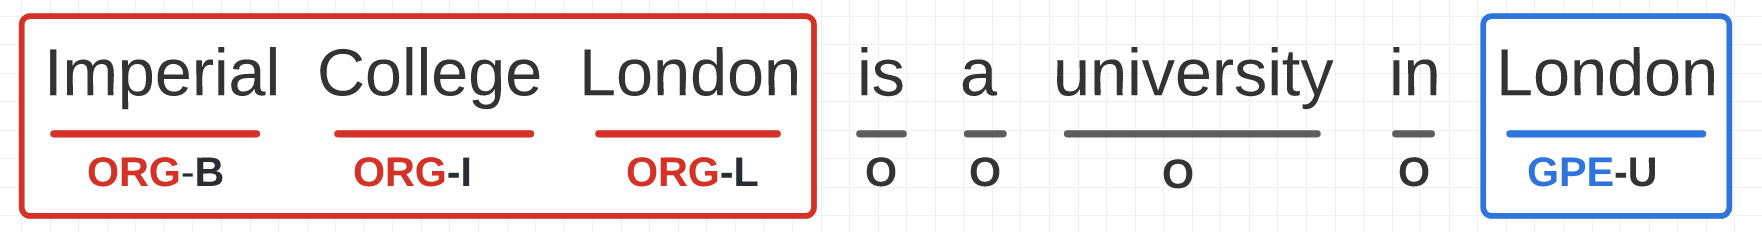
\includegraphics[scale=0.35]{images/bilou.png}
    \caption{NER using BILOU}
    \end{figure}

\subsubsection*{Conditional Random Fields}
A popular sequence labelling model is \textbf{Conditional Random Fields }(CRF). These are ``discriminative models" and generally outperform other Markov Models and such as Hidden Markov Models (HMM) as they are better able to cope with unseen tokens/words as well as Maximum Entropy Markov Models (MEMM) as they do not have labelling bias~\cite{crf}.

They work by maximising the log-likelihood of the posterior distribution $P(s|o)$ where $s$ is the output label sequence and $o$ is the observed input sequence. Let $s'$ denote the correct label sequence: 

\[ s' = \argmax_{s} P (s|p) \]

Therefore, it is fairly simple to determine output label sequence as it will be the one with the highest posterior probability. E.g., P([PER, ORG, ORG] | [Obama, UN, Congress]) will have a much higher probability than  P([LOC, LOC, LOC] | [Obama, UN, Congress])~\cite{crf}, where `PER', `LOC', `ORG' refers to person, location and organisation respectively.

The NER models are usually trained on specific domains and thereby only extract certain pre-defined types of entities such as PER, LOC, ORG etc. (See Appendix~\Cref{appendix:semantic_types}), thereby making them domain-dependent.

% \subsection{NER Approaches}

% \begin{enumerate}
%     \item \textbf{Rule $/$ knowledge-based approaches:} These methods depend on pre-defined (hand-crafted rules). The primary advantage is the lack of need for annotated training data as they focus on lexical representation and resources. These can be useful for domain-specific uses as they are rules are exhaustive and can help extract model-specific knowledge, resulting in high precision model. A drawback, however, is they will perform poorly when extended to other domains, and poor generalisability means constructing and maintaining lexicon resources for many domains is costly.

%     \item \textbf{Learning-based approaches:} These methods replace the human-curated rules. These methods can be further classed
% into three types: supervised, semi-supervised, and unsupervised. Supervised and semi-supervised methods,
% require the ML model to be trained on the input input given the corresponding output data to learn the features mapping the inputs to the outputs. Common examples to model the classifiers include  Hidden Markov Models (HMM), Support Vector Machines (SVM), and
% Conditional Random Fields (CRF). The type of classifier can have an effect on the accuracy of the NER task. For instance, SVM and HMM do not consider the dependencies among words. The unsupervised,
% bootstrapped methods are generally more automated in that they do not require an expansive training set (seeds) and but are less common. 
% (seeds). \hyperlink{9}{[9]}

% \item \textbf{Feature-inferring neural-network approaches:} Like learning-based approaches they incorporate machine learning techniques, however, they automatically infer the features by using deep neural networks (DNNs) such as LSTM. Reportedly, \hyperlink{9}{[9]}, they generally outperform the other approaches. They are able to perform feature extraction in the lower layers of the network and use these to train the classifier. The advantage is that they do not require seeds, ontologies or any domain-specific lexicons and are therefore domain-independent making them more robust. However, they do require huge datasets to build a decent model.  \hyperlink{9}{[9]}
% \end{enumerate}

\subsection{Named Entity Disambiguation and Linking}

\textbf{Named Entity Disambiguation (NED)}: NER might not always be able to classify a named identity due to it having a different meaning in different contexts. This is why named entity disambiguation is crucial to determine which
named entity a mention refers to; For instance, `Trump' can refer to either a person, a corporation or a building~\cite{ieee_named_entity}.

A common approach for disambiguating entities is to use context representation using the entirety of the text to find co-occurrence of `entity mentions' to establish `candidate' entities and use an existing knowledge base through `Named Entity Linking' to learn about the entities. The information from the knowledge can be used in conjunction with candidate-entity ranking approaches can be used which involve ranking candidate entries and retrieving the one with the highest probability for a target mention. 
An example in~\cite{ned}(p.7) shows that for the sentence: ``Michael Bloomberg is the mayor of New York", their algorithm correctly identifies New York in USA instead of London as `Michael Bloomberg' co-occurs in the same paragraph as `New York' (in USA) ``(88 times) more than with the New York in England (0 times)'' in the knowledge base. Quantifying  the impact of co-occurrences, can be done by using incidence matrix represents a weighted graph where weights are the co-occurrence $|$P(e$_{i}$,s,e$_{j}$,t)$|$ i.e. count of paragraphs, where two different entities e$_{i}$ and e$_{j}$ were mentioned together in two different sentence forms (s $\neq$ t)~\cite{ned}. 

Additionally, \textbf{Named Entity Linking (NEL)} uses a standard (unique) International Resource Identifier (IRI)~\cite{internationalized} for each disambiguated entity as described in a Knowledge Base (say, Linked Open Data (LOD) Cloud). Entity mentions are annotated by some NER algorithms, but they are restricted to the pre-defined types (such as persons, locations, organizations)~\cite{ieee_named_entity}. Knowledge base (KB) hosts millions of entities and therefore NEL can be used to ground mentions of entities in some text to a central KB. An example mentioned in~\cite{nel} highlights this: ``David Murray recruited from Positive Black Soul'' grounds Wikipedia articles for `David Murray' (saxophonist) but not the `David Murray' (musician) (disambiguation based on context). 
    
% \end{enumerate}

% \subsection{Named Entity Linking (NEL)}

% \textbf{Named Entity Linking (NEL)} aims to provide a standard IRI for each disambiguated entity as described in a Knowledge Base (e.g. Linked Open Data (LOD) Cloud). Entity mentions are annotated by some NER algorithms, but they are restricted to the pre-defined types (such as persons, locations, organizations). \hyperlink{9}{[9]} Knowledge base hosts millions of entities and therefore NEL can be used to ground mentions of entities in some text to a central KB. An example mentioned in this \hyperlink{14}{paper [14]}  highlights this: 'David Murray recruited from Positive Black Soul' grounds Wikipedia articles for David Murray (saxophonist) but not the David Murray (musician) (disambiguation based on context) and Positive Black Soul. 

% NEL has three main sub-tasks:

% \begin{enumerate}
%     \item Candidate-entity generation: tries to extract all possible entities in the knowledge base (KB) that could potentially refer to an entity mention in the text. This can be done by dictionary-based approaches, supervised learning of surface (sentence) form expansion from documents or probability-based approaches. 
    
%     \item Candidate-entity ranking: this step resembles disambiguation as seen in NED. This involves ranking candidate entries and retrieving the one with the highest probability for a target mention. The ranking can be established  via supervised methods (which include graph-based, model ensemble and probabilistic approaches) as well as unsupervised methods (which include Vector-Spaced Model and Information Retrieval based approaches.) \hyperlink{9}{[9]}
    
%     \item NIL clustering: handles those mentions in the text that have no matches with any entities in the knowledge base (KB). Of the three steps, this one is often not developed extensively. This can be implemented using string matching (grouping entities based on the string),  graph-based approaches (use a semantic entity graph) and hierarchical agglomerative clustering (based on minimising a distance metric). \hyperlink{9}{[9]}


%     \end{enumerate}
    
    
% \begin{figure}[H]
% \centering
% 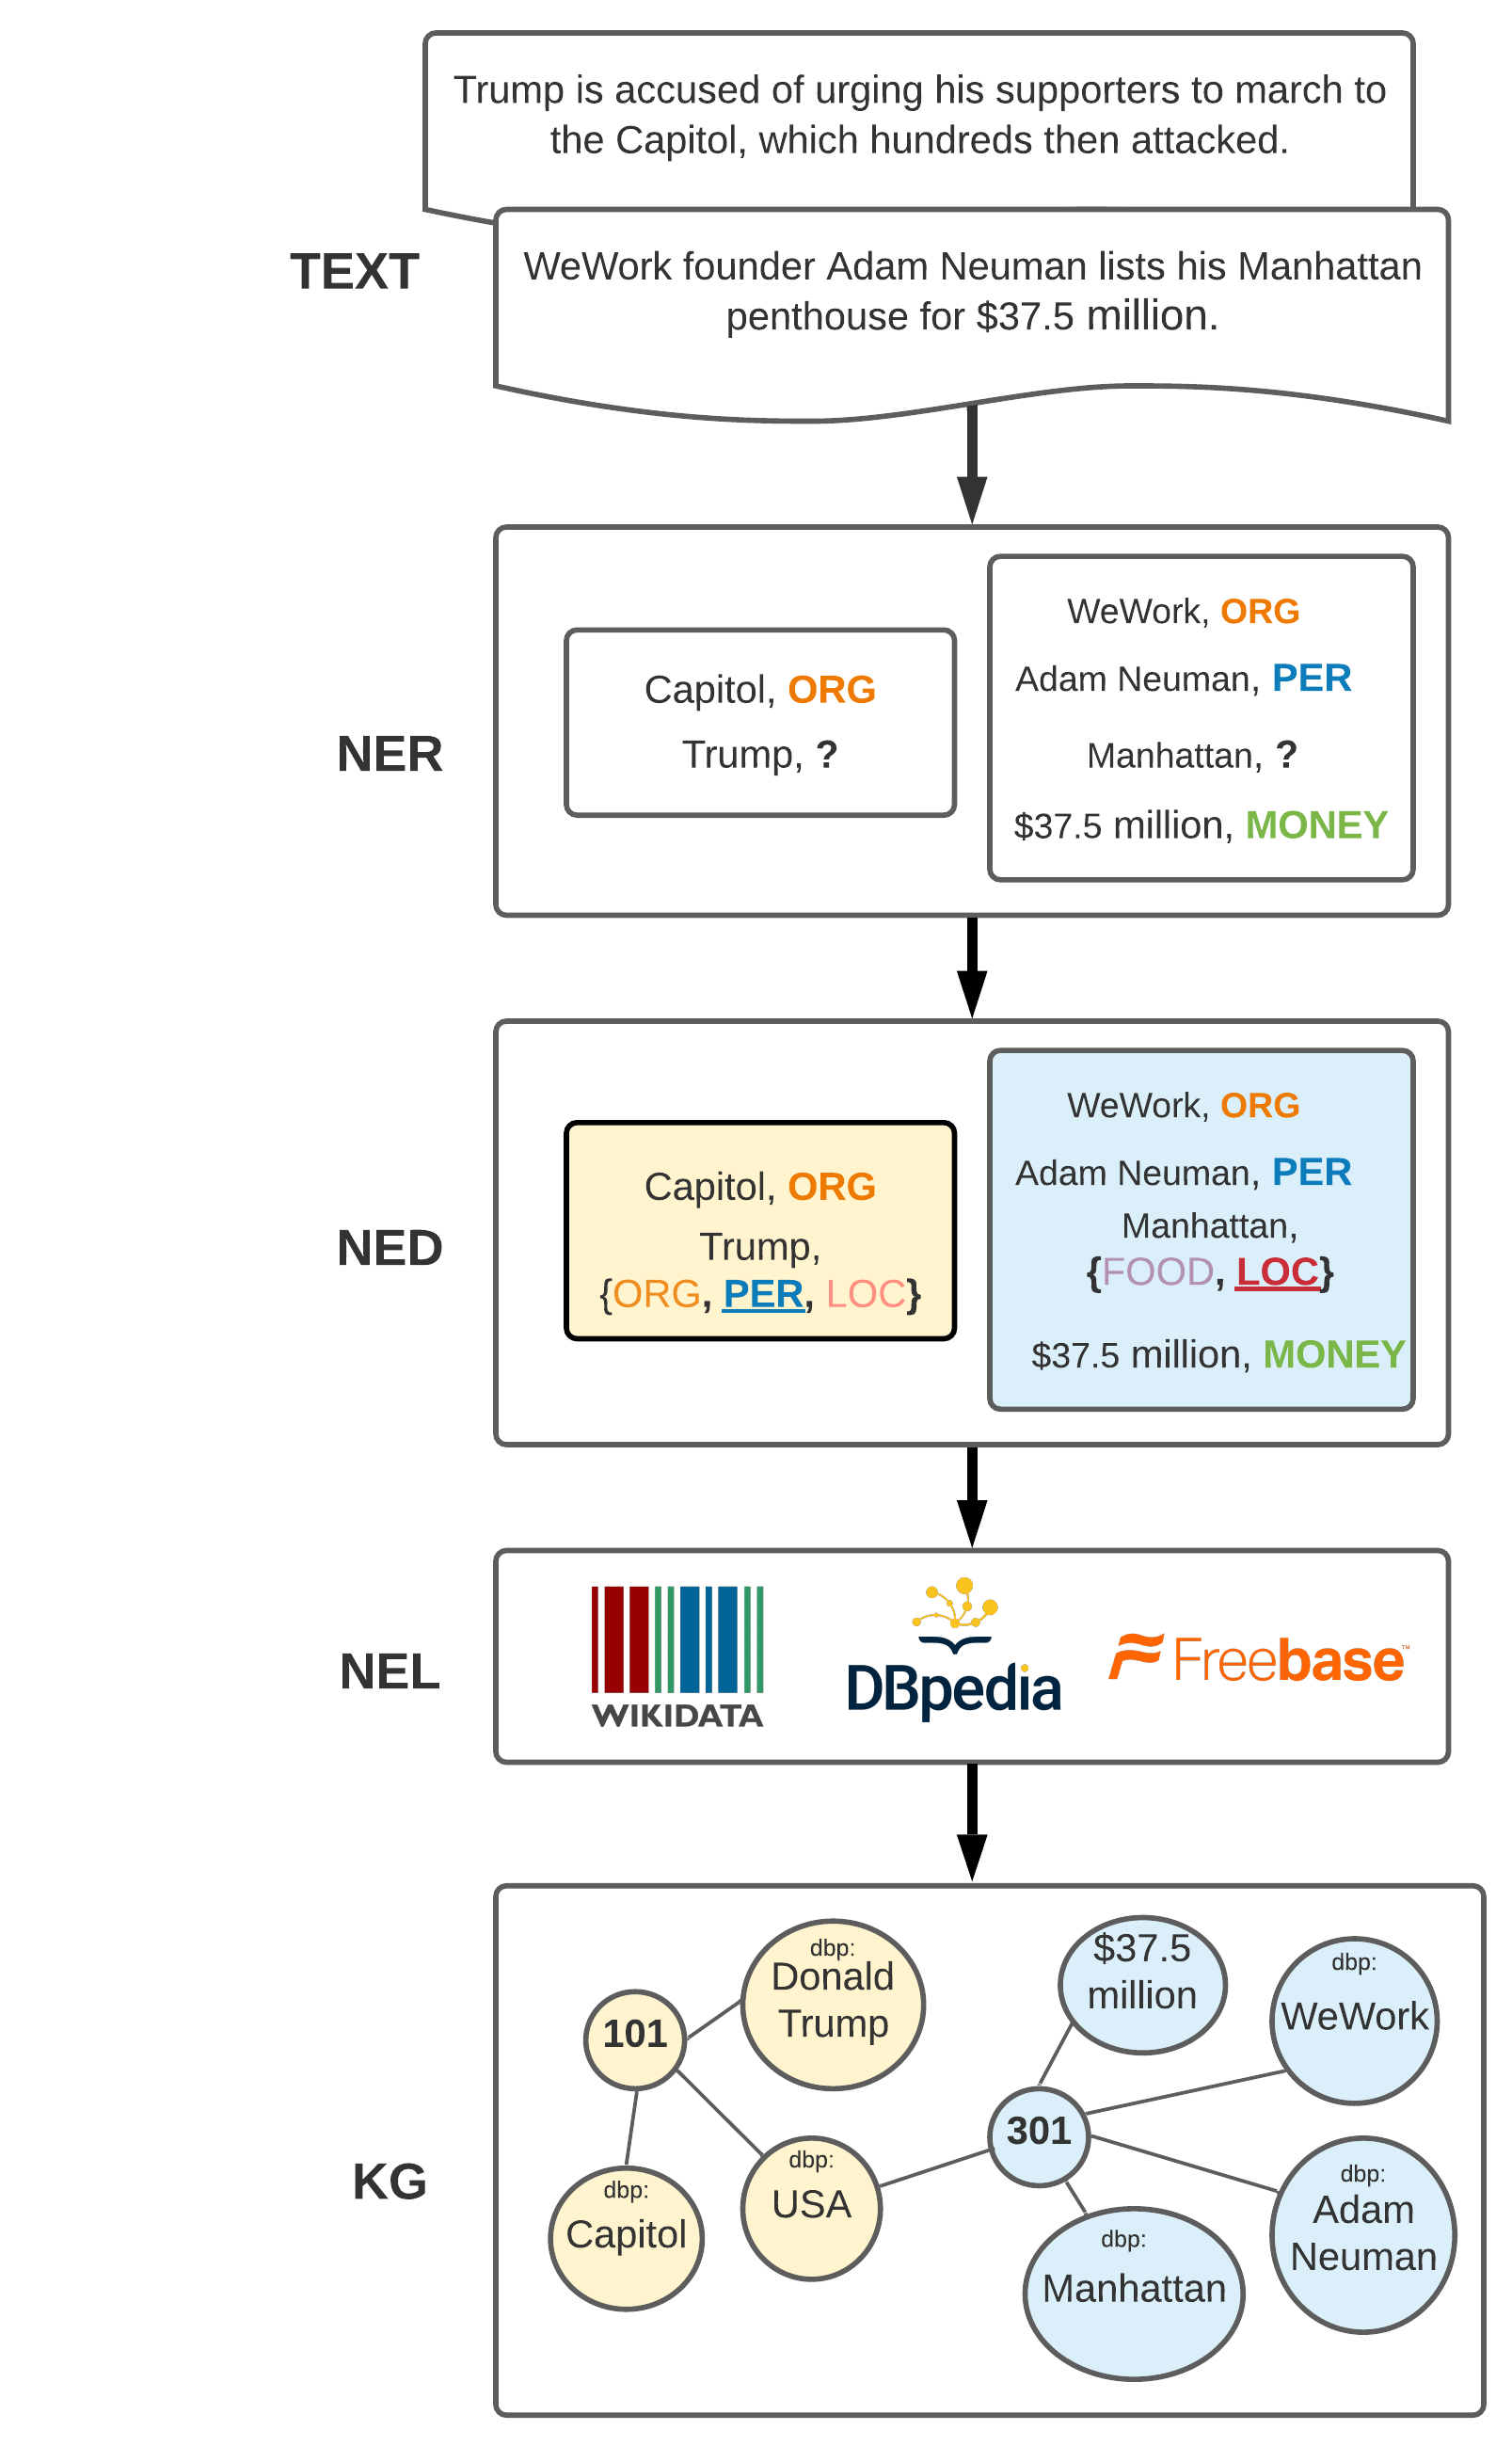
\includegraphics[scale = 0.2]{images/pipeline.png}
% \caption{Named Entity Extraction}
% \end{figure}